%%%% Better Poster latex template example v1.0 (2019/04/04)
%%%% GNU General Public License v3.0
%%%% Rafael Bailo
%%%% https://github.com/rafaelbailo/betterposter-latex-template
%%%% 
%%%% Original design from Mike Morrison
%%%% https://twitter.com/mikemorrison

\documentclass[a0paper,fleqn]{betterposter}

\usepackage{bm}
\usepackage{amsmath}

% print to the terminal the size of the main and side columns
\typeout{}
\typeout{--- Column dimensions ---}
\typeout{}
\typeout{Main column width: \the\dimexpr 1.0\textwidth-\leftbarwidth-\rightbarwidth\relax}
\typeout{Left column width: \the\leftbarwidth}
\typeout{Right column width: \the\rightbarwidth}
\typeout{1 pt = 1/864 printer's foot (249/250 standard foot) ~1/72.27 in}
\typeout{}
\typeout{-------------------------}
\typeout{}

%%%% Uncomment the following commands to customise the format

%% Setting the width of columns
% Left column
%\setlength{\leftbarwidth}{0.25\paperwidth}
% Right column
%\setlength{\rightbarwidth}{0.25\paperwidth}

%% Setting the column margins
% Horizontal margin
%\setlength{\columnmarginvertical}{0.05\paperheight}
% Vertical margin
%\setlength{\columnmarginhorizontal}{0.05\paperheight}
% Horizontal margin for the main column
%\setlength{\maincolumnmarginvertical}{0.15\paperheight}
% Vertical margin for the main column
%\setlength{\maincolumnmarginhorizontal}{0.15\paperheight}

%% Changing font sizes
% Text font
%\renewcommand{\fontsizestandard}{\fontsize{28}{35} \selectfont}
% Main column font
%\renewcommand{\fontsizemain}{\fontsize{28}{35} \selectfont}
% Title font
%\renewcommand{\fontsizetitle}{\fontsize{28}{35} \selectfont}
% Author font
%\renewcommand{\fontsizeauthor}{\fontsize{28}{35} \selectfont}
% Section font
%\renewcommand{\fontsizesection}{\fontsize{28}{35} \selectfont}

%% Changing font sizes for a specific text segment
% Place the text inside brackets:
% {\fontsize{28}{35} \selectfont Your text goes here}

%% Changing colours
% Background of side columns
%\renewcommand{\columnbackgroundcolor}{black}
% Font of side columns
%\renewcommand{\columnfontcolor}{gray}
% Background of main column
%\renewcommand{\maincolumnbackgroundcolor}{empirical}
%\renewcommand{\maincolumnbackgroundcolor}{theory}
%\renewcommand{\maincolumnbackgroundcolor}{methods}
%\renewcommand{\maincolumnbackgroundcolor}{intervention}
% Font of main column
%\renewcommand{\maincolumnfontcolor}{gray}
\newcommand{\source}{\mathrm{\bf{S}}}
\newcommand{\target}{\mathrm{\bf{T}}}
\newcommand{\D}{\mathcal{D}}
\newcommand{\nn}{\bm \Phi}
\newcommand{\sourceD}{\D^\source}
\newcommand{\targetD}{\D^\target}
\newcommand{\sourceNN}{\nn^\source}
\newcommand{\targetNN}{\nn^\target}
\newcommand{\f}{\mathrm{\bf{f}}}
\newcommand{\fSource}{\f^\source}
\newcommand{\fTarget}{\f^\target}
\newcommand{\footnoteSize}{\fontsize{18}{20} \selectfont}

\usepackage{tikz}

\begin{document}	
\betterposter{
%%%%%%%% MAIN COLUMN

\maincolumn{
%%%% Main space
% Transfer-Learning techniques \textbf{improve generalization} performance of data-driven models by adapting an existing source model to a similar target system with limited data.
% When training data is limited, adapting an existing model from a similar source system to the system of interest decreases model generalization error compared to training on the limited data alone.
% When training data is limited, adapting an \textbf{existing model} from a \textbf{similar system} to the system of interest \textbf{decreases model generalization error}.    
\textbf{Small changes} to an existing neural-network model can
\\accurately represent a
\\similar system using \textbf{less data} than initial training.
\vfill
\begin{center}
    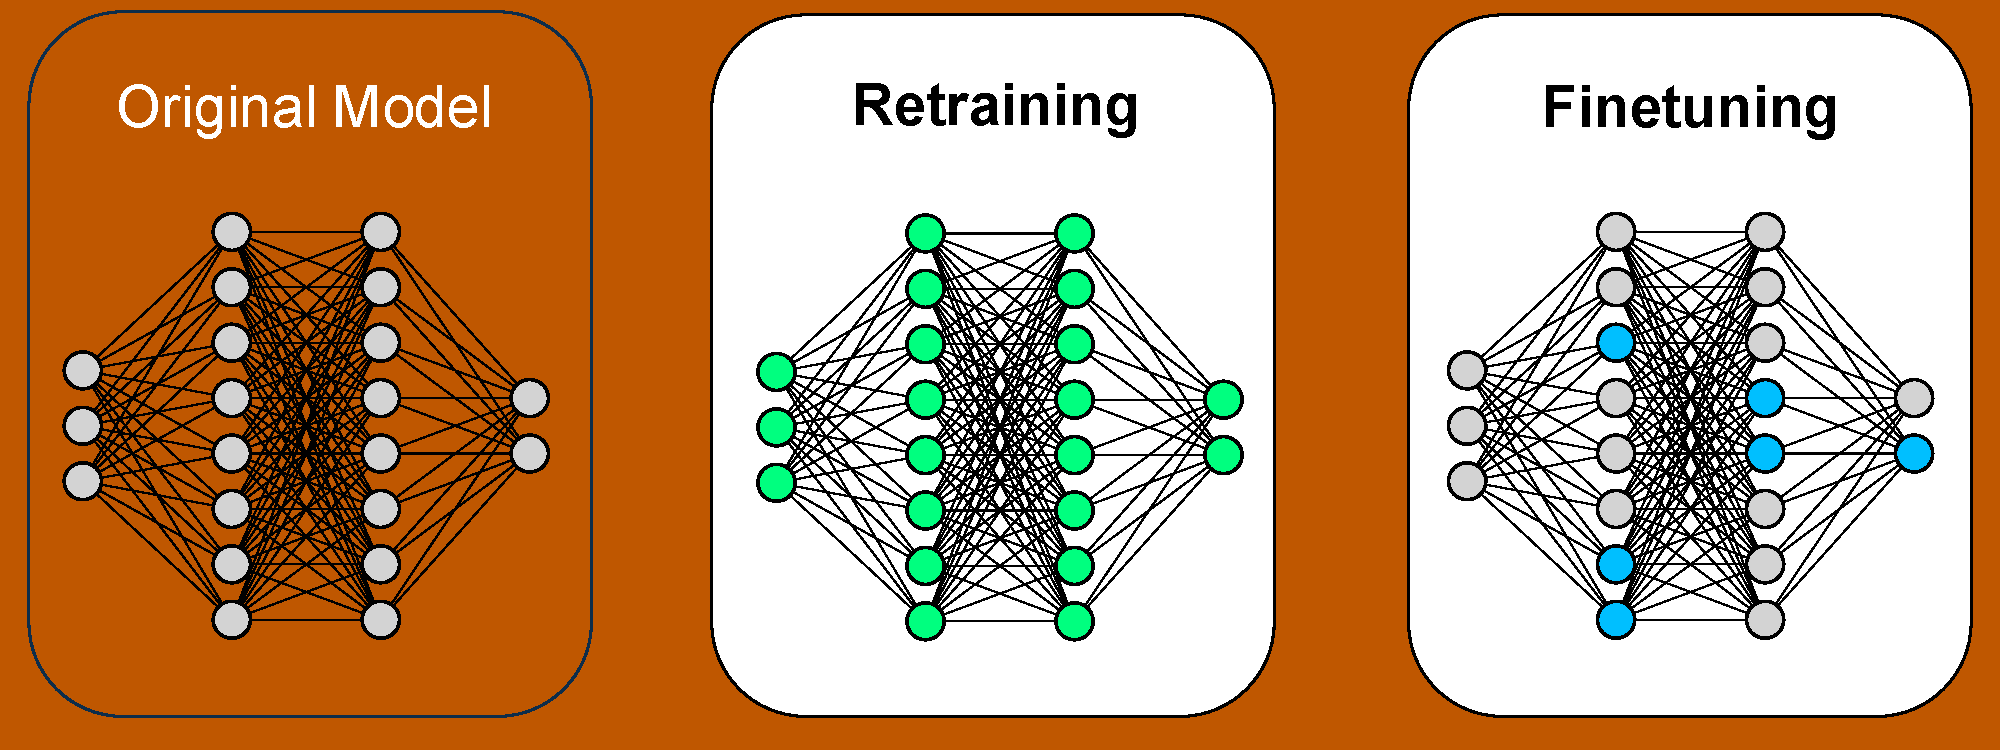
\includegraphics[width=\textwidth]{img/modelRetraining.pdf}
\end{center}
% \vfill
}{
%%%% Bottom space

%% QR code
\qrcode{img/qr.png}{img/smartphoneWhite}{
\textbf{Take a picture} or visit 
\\\textbf{bit.ly/TWCCC-Transfer-Learning}:
\begin{enumerate}
    \item Full results and presentation
    \item Previous work updating data-driven models of slowly-evolving dynamical systems
\end{enumerate}
}
% Smartphone icon
% Author: Freepik
% Retrieved from: https://www.flaticon.com/free-icon/smartphone_65680

%% Compact QR code (comment the previous command and uncomment this one to switch)
% \compactqrcode{img/qrcode}{
% \textbf{Take a picture} to
% \\download the full paper
% }

}

}{
%%%%%%%% LEFT COLUMN
\begin{center}
\title{Some Preliminary Transfer Learning Results for Dynamical Systems}
\end{center}
\author{Joshua E. Hammond, \\ Brian A. Korgel, Michael Baldea}
\institution{The University of Texas at Austin}
\author{Tyler A. Soderstrom}
\institution{ExxonMobil Technology and Engineering}

% \textbf{Objective:} Use limited data $\targetD$ from a target system $\fTarget$ and the model $\sourceNN$ of a similar source system $\fSource$ trained on abundant source data $\sourceD$ to learn an accurate model $\targetNN$ of the target system.
\textbf{Objective:} Use limited data from a target system and the model of a similar source system trained on abundant source data to learn an accurate neural-network representation of the target system.

% \textbf{Hypothesis:} If the source $\source$ and target $\target$ systems are sufficiently similar, in the data space, and the functional space:
\textbf{Hypothesis:} If $\f^\source\leftrightarrow\f^\target$ and $\sourceD\leftrightarrow\targetD$:
\begin{enumerate}
    \item The parameter space of $\sourceNN$ is close to that of $\targetNN$.
    \item A path exists from the source model parameters to the target model parameters.
\end{enumerate} 

\section{Spring-Mass-Damper System}
$m\ddot{x} + c\dot{x} + kx = u$\\
\textbf{Given:} $x_0$, $\dot{x}_0$ \hspace{3em} \textbf{Predict:} $x_1, \ldots , x_{20}$\\
\textbf{Transfer:} $m,c,k,u\pm10\%$\\
$\dim(\sourceD)=100,000$, $\dim(\targetD)=1,000$

\begin{center}
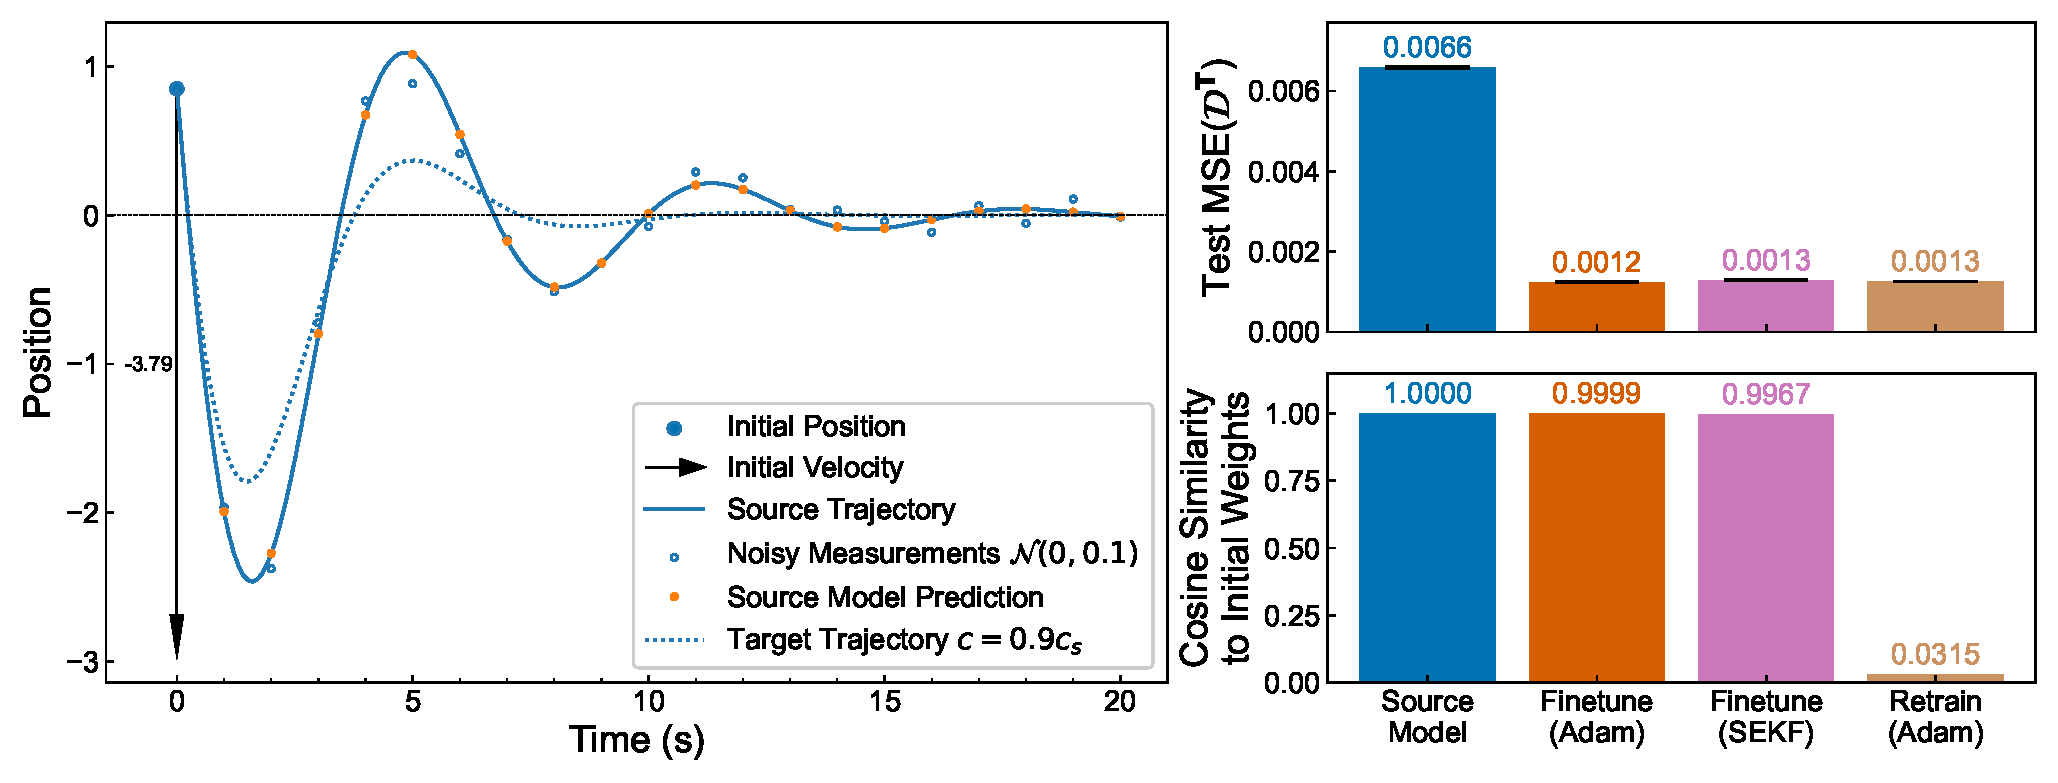
\includegraphics[width=\textwidth]{img/springResults}
\end{center}

\section{CSTR System$^\mathrm{[1]}$}
$A \rightarrow B \rightleftharpoons C$\\
\textbf{Given:} $C_{A,0}, C_{B,0}, C_{C,0}, C_{Af,0 \ldots 59}$ \hspace{1em} \\\textbf{Predict:} $C_{A,1 \ldots 60}, C_{B,1 \ldots 60}, C_{C,1 \ldots 60}$\\
\textbf{Transfer:} $\Delta V_{rxn} -20\%$\\
$\dim(\sourceD)=1 \text{ Year}, \dim(\targetD)=1\text{ Day}$
\begin{center}
    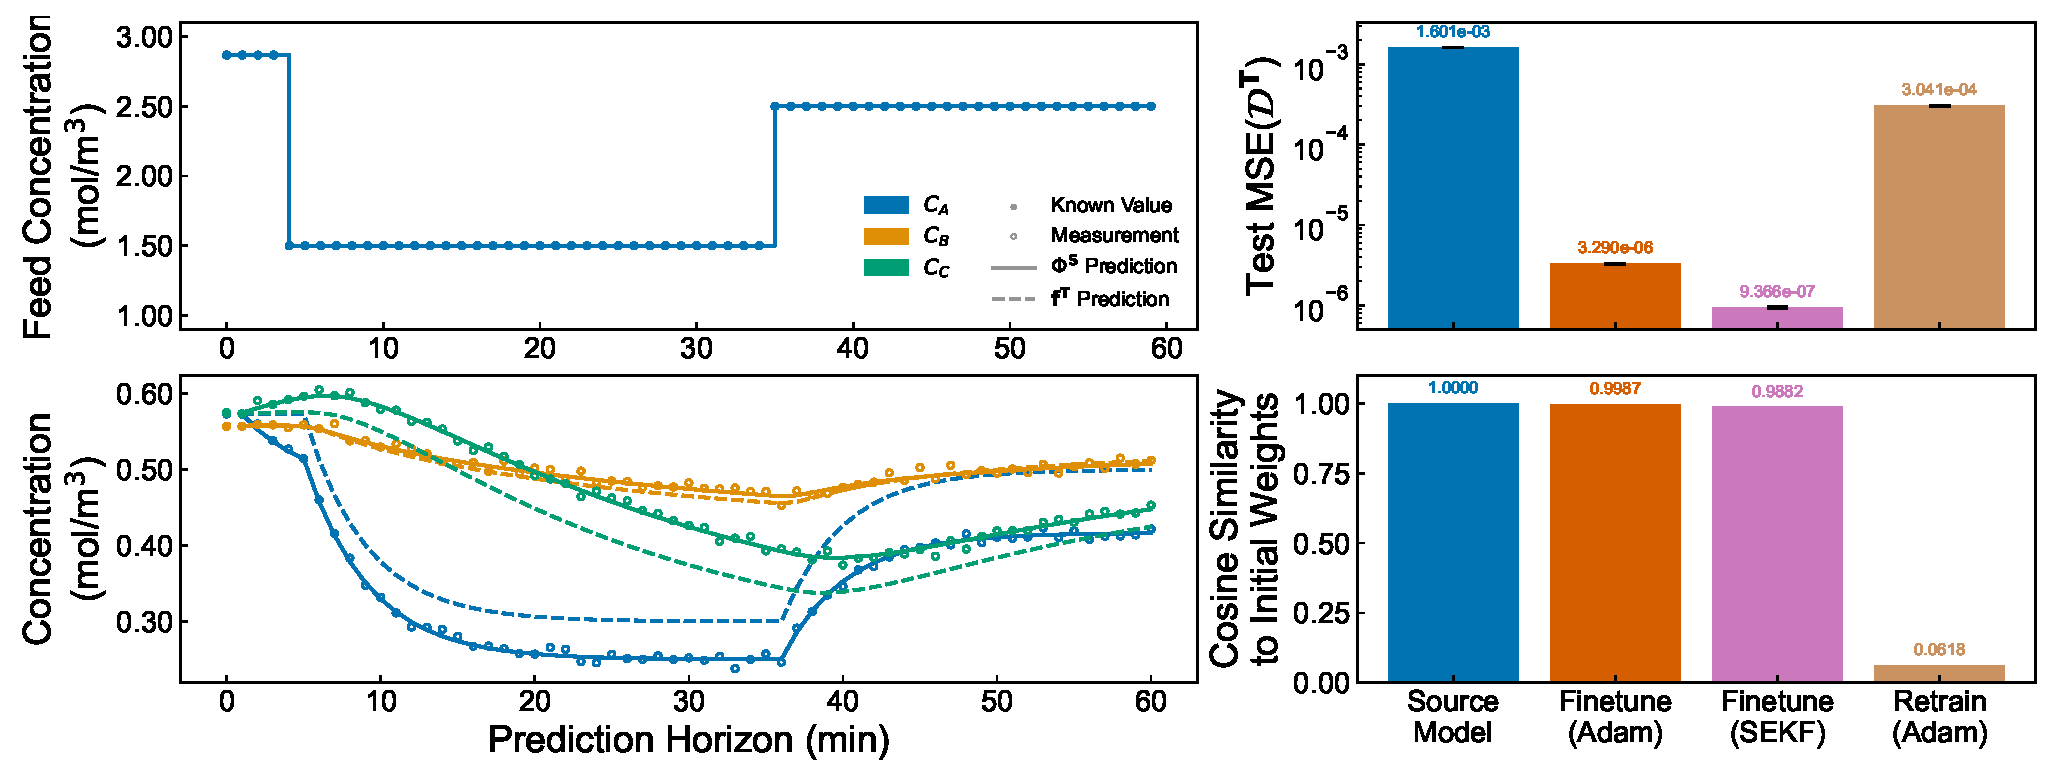
\includegraphics[width=\textwidth]{img/CSTRResults}
\end{center}

% %% This fills the space between the content and the logo
% \vfill

% {\fontsize{18}{19} \selectfont [1] Kumar, P., \& Rawlings, J. B. (2023). Structured nonlinear process modeling using neural networks and application to economic optimization.\ \textit{Computers and Chemical Engineering}, 177. %\href{https://doi.org/10.1016/j.compchemeng.2023.108314}{https://doi.org/10.1016/j.compchemeng.2023.108314}

% [1] Kumar, P., \& Rawlings, J. B. (2023). Structured nonlinear process modeling using neural networks and application to economic optimization. \textit{Computers and Chemical Engineering}, 177. %\href{https://doi.org/10.1016/j.compchemeng.2023.108314}{https://doi.org/10.1016/j.compchemeng.2023.108314}

{\footnoteSize [1] Kumar, P., \& Rawlings, J.B. (2023). Structured nonlinear process modeling using neural networks and application to economic optimization. %\href{https://doi.org/10.1016/j.compchemeng.2023.108314}{https://doi.org/10.1016/j.compchemeng.2023.108314}
\par
}

}{
%%%%%%%% RIGHT COLUMN
\vfill

\section{Machine Learning Models of Dynamical Systems}
$\frac{d\bf{x}}{dt} = \f^\source(\bf{x}, \bf{u}, \bf{p^\source})$
\hspace{5em} ${\bf{x}_{k+1}} = {\bf{\Phi}^\source(\bf{x}_k, \bf{u}_k,} \bm{\pi}^\source)$\par
$\frac{d\bf{x}}{dt} = \f^\target(\bf{x}, \bf{u}, \bf{p^\target})$
\hspace{5em} ${\bf{x}_{k+1}} = {\bf{\Phi}^\target(\bf{x}_k, \bf{u}_k,} \bm{\pi}^\target)$\par
% \end{center}

% \section{Transfer Learning}
% \begin{center}
% 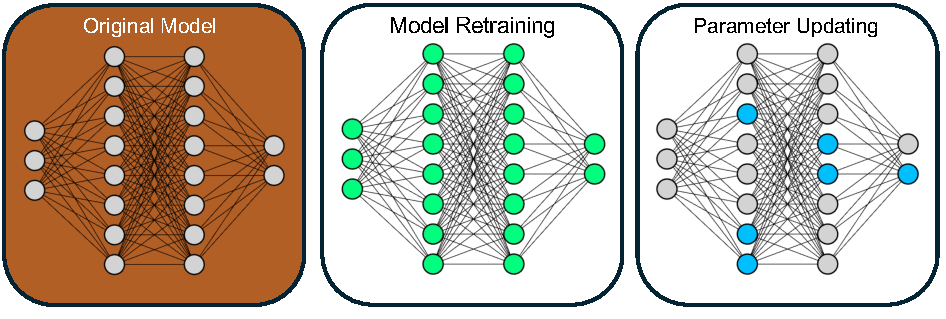
\includegraphics[width=0.8\textwidth]{img/Methods.pdf}
% \end{center}
% In transfer learning, we begin with the parameters $\bm{\pi}^\source$ of a pre-trained source model $\sourceNN$.
\vfill
\section{Defining Similarity}
% \vspace{-2em}
% \begin{itemize}
%     \item[] \textbf{Data Space Similarity:} The input and output data of $\sourceD$ and $\targetD$ have similar ranges and distributions.
%     \item[] \textbf{Functional Space Similarity:} The governing equations $\fSource$ and $\fTarget$ have similar forms and parameters. Similarly, given the same input, $\sourceNN$ and $\targetNN$ produce similar output trajectories.
%     \item[] \textbf{Representation/Parameter Similarity:} The internal representations of the NN model, embeddings, or model parameters are similar.
% \end{itemize}
We use \textit{cosine similarity} to quantify the similarity of individual NN outputs and the weights of two NNs

\begin{center}
    
\includegraphics[width=0.8\textwidth]{img/cosineSimilarity}
\end{center}

$\text{cosine\_similarity}\left(\bf{a}, \bf{b}\right) \triangleq \cos(\theta) = \frac{\bf{a} \cdot \bf{b}}{\|\bf{a}\| \|\bf{b}\|} \in [-1,1]$
\vfill
\section{The Subset Extended Kalman Filter (SEKF)$^\mathrm{[2]}$}
\vspace{-2em}
\begin{center}
    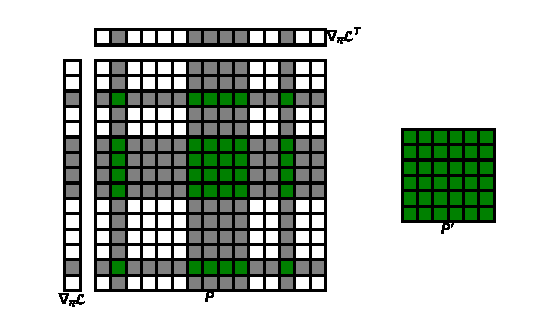
\includegraphics[width=0.7\textwidth]{img/subset_matrices_mpl}
\end{center}

The SEKF reduces the computational cost of EKF operations by only updating a subset of the NN model parameters $\bm{\pi}$ at each time step. We use the gradient of the loss function with respect to the parameters $\nabla_{\bm{\pi}}\mathcal{L}$ to select which subset of parameters to update.
\\The gradients of the selected parameters along with the corresponding subset of the covariance matrix $\bf{P}$ are used in the EKF update equations.

\vspace{12pt}

{\footnoteSize [2] Hammond et. al ``Staying Alive: Online Neural Network Maintenance and Systemic Drift'' arXiv:2503.17681
\par
}

\vfill

\section{Nomenclature}

\vspace{-2em}
\begin{tabular}{ll|ll}
    $\source$ & Source & $\target$ & Target \\
    $\f$ & Governing Equations & $\D$ & Dataset \\
    $\nn$ & Neural Network & $\bf{x}$  &  States \\
    $\bf{u}$ & Inputs & $\bf{p}$ & System Parameters \\
    $\bm{\pi}$ & NN parameters & $\nabla_{\bm{\pi}}\mathcal{L}$ & Gradient of Loss Function w.r.t. $\bm{\pi}$ \\
\end{tabular}

\vspace{1em}

%% Institution logo
\begin{center}
% 
\includegraphics[width=0.8\textwidth,trim={1.8cm 2cm 1cm 0}]{img/RGB_university_primary}\\

\includegraphics[width=0.7\textwidth,trim={0 0 0 0}]{img/Cockrell_RGB_formal_CHE}
\end{center}
}
\end{document}
